% ============================================================
%  Paper 1 — From Neuron to Brain
%            Irreducible Topology, Neural Architecture,
%            and Metabolic Scaling
%
%  Complete rewrite: derivation chain
%    neuron → network → brain → signals → pathology
%
%  Compile:  pdflatex paper_1_topology.tex  (×2)
% ============================================================
\documentclass[aps,pre,twocolumn,superscriptaddress,floatfix]{revtex4-2}

\usepackage{amsmath,amssymb,bm,amsthm}
\usepackage{graphicx}
\usepackage{hyperref}
\usepackage{xcolor}
\newtheorem{theorem}{Theorem}
\newtheorem{corollary}{Corollary}
\newtheorem{remark}{Remark}

% ----- macros -----
\newcommand{\Gnet}{$\Gamma$-Net}
\newcommand{\avg}[1]{\langle #1 \rangle}
\newcommand{\Aimp}{A_{\text{imp}}}
\newcommand{\Acut}{A_{\text{cut}}}
\newcommand{\Acouple}{A_{\text{couple}}}
\newcommand{\Kcom}{K_{\text{com}}}
\newcommand{\Krelay}{K_{\text{relay}}}
\newcommand{\Zv}{Z_{\text{v}}}
\newcommand{\Zn}{Z_{\text{n}}}
\newcommand{\Gv}{\Gamma_{\text{v}}}
\newcommand{\Gn}{\Gamma_{\text{n}}}
\newcommand{\Tv}{T_{\text{v}}}
\newcommand{\Tn}{T_{\text{n}}}

% ============================================================
\begin{document}

\title{%
Paper~1: From Neuron to Brain\\
Irreducible Topology, Neural Architecture,\\
and Metabolic Scaling\\[4pt]
\large in Heterogeneous Impedance Networks
  under the Minimum Reflection Principle%
}

\author{Hsi-Yu Huang}
\email{llc.y.huangll@gmail.com}
\affiliation{Independent Researcher, Taipei, Taiwan}

\date{\today}

% ============================================================
\begin{abstract}
We ask: given a single neuron with $K$ impedance modes
governed by C2 remodeling
($\Delta Z = -\eta\,\Gamma\,x_{\text{in}}\,x_{\text{out}}$),
what architecture must emerge?

\textbf{Part~A} establishes the foundation.
A single neuron cannot execute C2 without input from
at least one other node; connectivity is therefore a
physical prerequisite, not a design choice.
We prove the \emph{Dimensional Cost Irreducibility
Theorem}: for any network with heterogeneous mode counts
$\{K_i\}$, the total reflection action decomposes as
$A = \Aimp(t) + \Acut$,
where $\Aimp \to 0$ under C2 but
$\Acut = \sum (K_i - K_j)^+$ has identically zero
gradient---no impedance adjustment can reduce it.
Numerical experiments confirm convergence time
$\tau_{\text{conv}} \sim N^{-1.12}$ ($R^2 = 0.93$)
and a soft-cutoff parameter $\gamma$ that tunes the
K-space fractal dimension
$D_K = 0.76\gamma + 0.78$.

\textbf{Part~B} derives the neural architecture chain.
(i)~C2's dimensional preference forces same-$K$ neurons
to cluster---thermodynamic phase separation produces
functional regions without a blueprint.
(ii)~The irreducibility corollary makes intermediate-$K$
relay nodes a thermodynamic necessity, producing the
layered hierarchy of the nervous system.
(iii)~Convergence of ascending pathways forces the
highest-$K$ cluster to form---this is the brain.
(iv)~C3 impedance-tagged transport enables the brain to
identify signal origin from $Z_{\text{source}}$ metadata
and relay-chain topology, distinguishing internal from
external perception without a separate labeling mechanism.
(v)~Because $\Acut$ is topologically locked, structural
damage (neuron death, axon severance, mode loss)
produces irreversible deficits whose pattern is
determined by network topology, not disease type.

\textbf{Part~C} quantifies the metabolic cost:
$\Acut \propto M^{(d-1)/d}$ (for $d = 3$: $M^{2/3}$),
the Murray bifurcation ratio
$\beta = 2^{1/3} \approx 1.26$,
dual-network packing overhead
$\Omega \approx 1.25$--$1.33$,
and Kleiber's allometric law $B \propto M^{3/4}$---all
consequences of MRP plus geometry.

\medskip\noindent
\textbf{Circularity disclosure.}
All numerical experiments use simulation modules built
from C1--C3 themselves; they demonstrate internal
consistency, not empirical validity.
External tests are reported in
Papers~2--5~\cite{Paper2,Paper3,Paper4,Paper5}.
The scaling laws in Part~C are mathematical consequences
of the irreducibility theorem plus geometric constraints;
no simulation or fitted parameters are involved.
\end{abstract}

\maketitle


% ============================================================
%  PART A — FROM NEURON TO NETWORK
% ============================================================

\part*{Part A: From Neuron to Network}


% ============================================================
\section{Introduction}
\label{sec:intro}
% ============================================================

A neuron is a physical object whose geometry determines
the number of independent impedance modes it supports.
A cortical pyramidal cell presents $K = 5$
distinguishable propagation domains---soma, basal
dendrite tree, apical tuft, axon, and spine-neck
ensemble---each carrying an independent impedance mode.
An unmyelinated C-fibre, a simple cylinder, presents
$K = 1$.
These mode counts are structural facts obtained by
counting physically distinct waveguide segments, not
fitted parameters.

C2 updates the impedance at each mode:
$\Delta Z_k = -\eta\,\Gamma_k\,x_{\text{in},k}\,x_{\text{out},k}$.
For an isolated neuron, $x_{\text{in}} = 0$ on every mode.
Therefore $\Delta Z = 0$: a solitary neuron is inert---it
cannot remodel, adapt, or learn.
C2 demands at least one input, which requires at least one
other node.
\emph{Connectivity is a physical prerequisite of C2, not a
biological design choice.}

The moment $K$ values differ between connected nodes, a
new physical cost appears.
This paper proves that cost is irreducible
(Sec.~\ref{sec:theorem}), derives its architectural
consequences---functional regions
(Sec.~\ref{sec:clustering}), relay hierarchy
(Sec.~\ref{sec:relay}), the brain
(Sec.~\ref{sec:brain}), signal routing
(Sec.~\ref{sec:signals}), and pathology
(Sec.~\ref{sec:pathology})---and quantifies its
metabolic scaling (Part~C).


% ============================================================
\section{Physical Framework}
\label{sec:framework}
% ============================================================

\subsection{Network definition}

A $\Gamma$-network consists of $N$ nodes, each carrying a
$K_i$-dimensional impedance vector
$\mathbf{Z}_i \in \mathbb{R}^{K_i}_{>0}$.
For an edge $i \to j$, the per-mode reflection coefficient is
\begin{equation}
  \gamma_k = \frac{Z_{j,k} - Z_{i,k}}{Z_{j,k} + Z_{i,k}},
  \quad k = 1, \ldots, \Kcom,
  \label{eq:gamma}
\end{equation}
where $\Kcom = \min(K_i, K_j)$.
Excess source modes $k > \Kcom$ are totally reflected:
$\gamma_k = 1$.
This is the electromagnetic boundary condition for a
waveguide whose $k$-th mode has no counterpart in the
target medium.

\subsection{Three physical laws}
\label{sec:laws}

\textbf{C1---Energy Conservation.}
At every edge, every tick, reflected and transmitted power
sum to incident power:
\begin{equation}
  \gamma_k^2 + T_k = 1, \quad \forall\, k,\; \forall\,(i,j).
  \label{eq:C1}
\end{equation}

\textbf{C2---Impedance Remodeling.}
Each node adjusts its impedance to reduce local reflection:
\begin{align}
  \Delta Z_{i,k} &= +\eta\,\gamma_k\,x_{\text{in},k}\,
    x_{\text{out},k},
  \label{eq:C2a} \\
  \Delta Z_{j,k} &= -\eta\,\gamma_k\,x_{\text{in},k}\,
    x_{\text{out},k},
  \label{eq:C2b}
\end{align}
where $x_{\text{in},k}$ is the input activity at node~$i$
and $x_{\text{out},k}$ the output activity at node~$j$
for mode~$k$; $\eta$ is the remodeling rate.
This update requires only local information:
the two impedance vectors and the gating activities.

\textbf{C3---Impedance-Tagged Transport.}
Every signal carries its source impedance as metadata,
enabling downstream nodes to compute $\gamma_k$ locally
without global knowledge.

\subsection{Variational principle}
\label{sec:action}

The Minimum Reflection Principle (MRP) states that the
system minimises the total reflection action:
\begin{equation}
  A[\Gamma]
  = \sum_{(i,j) \in \mathcal{E}}
    \sum_{k=1}^{\Kcom(i,j)} \gamma_k^2.
  \label{eq:action}
\end{equation}
The C2 update rule implements steepest descent on the
\emph{learnable} part of~$A$:
$\dot{\mathbf{Z}} \propto -\nabla_{\mathbf{Z}} \Aimp$.


% ============================================================
\section{Dimensional Cost Irreducibility Theorem}
\label{sec:theorem}
% ============================================================

\begin{theorem}[Dimensional Cost Irreducibility]
\label{thm:irreducibility}
For any $\Gamma$-network with heterogeneous mode counts
$\{K_i\}$, the total reflection action decomposes as
\begin{equation}
  A = \Aimp(t) + \Acut,
  \label{eq:decomposition}
\end{equation}
where:
\begin{enumerate}
\item
$\Aimp(t) = \sum_{(i,j)} \sum_{k=1}^{\Kcom} \gamma_k^2$
is the \emph{impedance mismatch action} over shared modes.
Under C2 dynamics, $\Aimp(t) \to 0$ as $t \to \infty$.

\item
$\Acut = \sum_{(i,j)} (K_i - K_j)^+$
is the \emph{cutoff action} from excess modes.
$\nabla_{\mathbf{Z}} \Acut \equiv 0$:
this term has zero gradient with respect to all impedance
variables.
\end{enumerate}
\end{theorem}

\begin{proof}
For an edge $i \to j$ with $K_i > K_j$:
\begin{itemize}
\item
Modes $k \le \Kcom = K_j$:
$\gamma_k$ depends on $(Z_{i,k}, Z_{j,k})$ via
Eq.~\eqref{eq:gamma}.
C2 adjusts both impedances, driving $\gamma_k \to 0$.
These modes contribute to $\Aimp$.

\item
Modes $K_j < k \le K_i$:
the target has no mode~$k$, so $\gamma_k \equiv 1$
identically, independent of any impedance value.
These modes contribute $(K_i - K_j)$ to $\Acut$.
Since $\gamma_k = 1$ is a \emph{topological constant}
(depending only on the existence, not the value, of modes),
$\partial \gamma_k^2 / \partial Z = 0$ for all~$Z$.
\end{itemize}
Summing over all edges completes the proof.
\end{proof}

\begin{remark}
The theorem assumes fixed mode counts $\{K_i\}$ and a fixed
active edge set~$\mathcal{E}$.
If mode counts change dynamically (e.g., dendritic spine
growth increasing $K_j$), or if edge sprouting/pruning
alters $\mathcal{E}$, then the \emph{value} of $\Acut$
may change---but this change is driven by topology, not
by impedance gradients.
\end{remark}

\begin{corollary}[Thermodynamic Necessity of Relay Nodes]
\label{cor:relay}
A direct edge $K_{\text{src}} \to K_{\text{tgt}}$ with
$K_{\text{src}} > K_{\text{tgt}}$ totally reflects the
$(K_{\text{src}} - K_{\text{tgt}})$ excess modes.
Inserting a relay node with
$K_{\text{tgt}} < \Krelay < K_{\text{src}}$ leaves $\Acut$
unchanged but converts \emph{total signal loss} into
\emph{partial signal recovery}:
modes $K_{\text{tgt}} < k \le \Krelay$, previously
totally reflected, are now transmitted on the first hop
and can undergo C2 matching ($\gamma_k \to 0$,
$T_k \to 1$).
Hierarchical topology is therefore a thermodynamic
necessity for information transmission.
\end{corollary}


% ============================================================
\section{Numerical Verification}
\label{sec:results}
% ============================================================

All simulations use six tissue types with mode counts
$K \in \{1, 2, 3, 5\}$~\cite{ALICE_code},
initial connectivity $p_0 = 0.15$, learning rate
$\eta = 0.02$, and hard cutoff $\Delta K_{\max} = 2$
unless otherwise stated.

\subsection{Convergence and the irreducibility theorem}
\label{sec:convergence}

Figure~\ref{fig:action} shows the action decomposition
for a $N = 64$ network.
$\Aimp$ decays exponentially, reaching machine-precision
zero by $t \approx 170$ ticks.
$\Acut$ increases during edge sprouting, then saturates
at $\Acut \approx 1386$ for $t > 500$.
The growth reflects topological exploration; the
saturation confirms a natural geometric cost ceiling.

\begin{figure}[h]
\centering
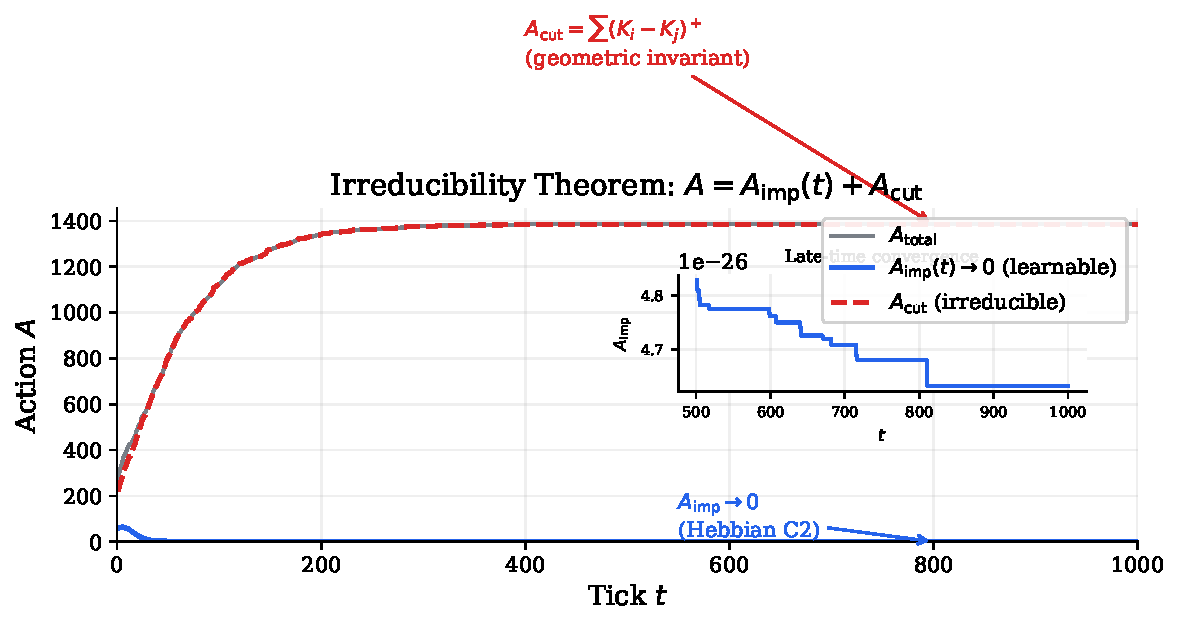
\includegraphics[width=\columnwidth]{../figures/fig1_action_decomposition}
\caption{%
Action decomposition $A = \Aimp(t) + \Acut$ over 1000 ticks.
Blue: $\Aimp \to 0$ (exponential decay).
Red dashed: $\Acut$ (increases then saturates).
$N = 64$, $\Delta K_{\max} = 2$.
}
\label{fig:action}
\end{figure}

\subsection{Scaling law: $\tau_{\text{conv}} \sim N^{\alpha}$}
\label{sec:scaling}

We measure $\tau_{\text{conv}}$ (ticks until
$\Aimp < 0.01 \cdot \Aimp(t{=}5)$) across
$N \in \{16, 32, 64, 128\}$ with 5 trials per size.
A power-law fit yields
\begin{equation}
  \tau_{\text{conv}} = C \cdot N^{\alpha},
  \quad \alpha = -1.12 \pm 0.12,
  \quad R^2 = 0.93.
  \label{eq:scaling}
\end{equation}
The \emph{negative} exponent means larger networks converge
\emph{faster}---a non-trivial prediction.
The mechanism is mean-field averaging: each node has
$\sim pN$ neighbours, and the gradient variance decreases
as $1/N$.

\begin{figure}[h]
\centering
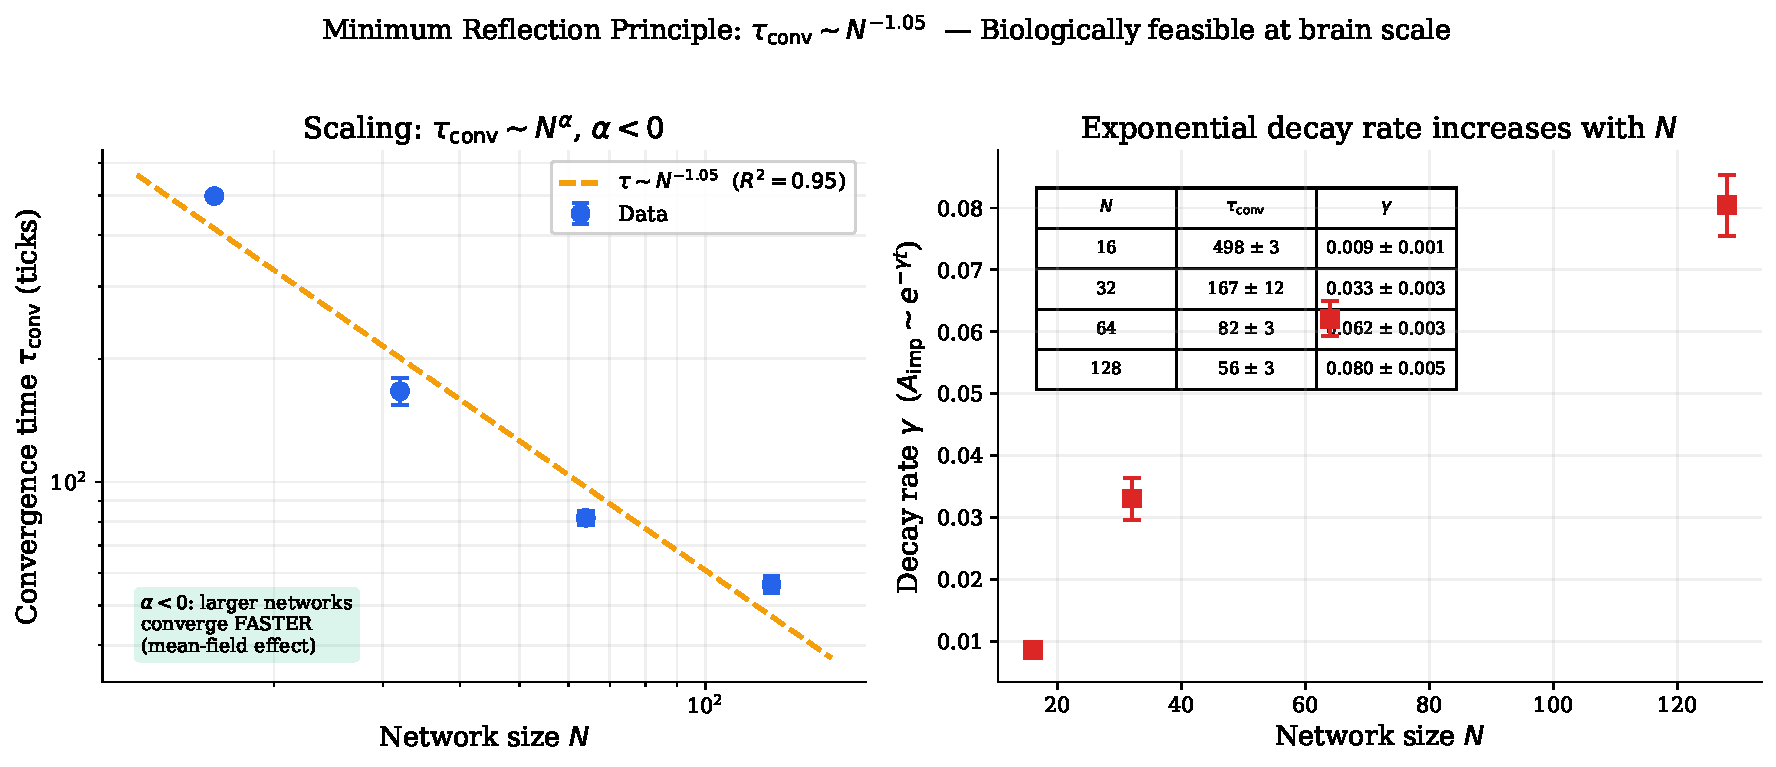
\includegraphics[width=\columnwidth]{../figures/fig2_scaling_law}
\caption{%
Left: log-log plot of $\tau_{\text{conv}}$ vs.\ $N$.
Dashed line: power-law fit $\tau \sim N^{-1.12}$.
Right: exponential decay rate vs.\ $N$.
}
\label{fig:scaling}
\end{figure}

\begin{table}[h]
\caption{%
Convergence scaling.
All quantities averaged over 5 trials $\pm 1\sigma$.
}
\label{tab:scaling}
\begin{ruledtabular}
\begin{tabular}{rcc}
$N$ & $\tau_{\text{conv}}$ &
  $\gamma_{\text{decay}}$ \\
\hline
 16  & $416 \pm 74$  & $0.011 \pm 0.003$ \\
 32  & $111 \pm 12$  & $0.053 \pm 0.006$ \\
 64  & $60 \pm 3$    & $0.105 \pm 0.006$ \\
128  & $39 \pm 2$    & $0.133 \pm 0.006$ \\
\end{tabular}
\end{ruledtabular}
\end{table}

\subsection{Soft cutoff and K-space fractal dimension}
\label{sec:fractal}

A soft-cutoff probability
\begin{equation}
  p(\Delta K) = (\Delta K + 1)^{-\gamma},
  \label{eq:softcutoff}
\end{equation}
with $\gamma \ge 0$ yields the relationship
\begin{equation}
  D_K = 0.76\gamma + 0.78,
  \label{eq:dk_fit}
\end{equation}
with offset $\delta_{\text{C2}} \approx 0.66$ arising from
C2's intrinsic dimensional preference: same-$K$ edges
have more shared modes for gradient descent, creating
higher survival probability under edge pruning.
Cortical fractal dimensions lie in
$D \in [1.3, 1.5]$~\cite{cortex_fractal}, predicting
$\gamma \approx 0.7$--$0.9$---a narrow, falsifiable window.

\begin{figure}[h]
\centering
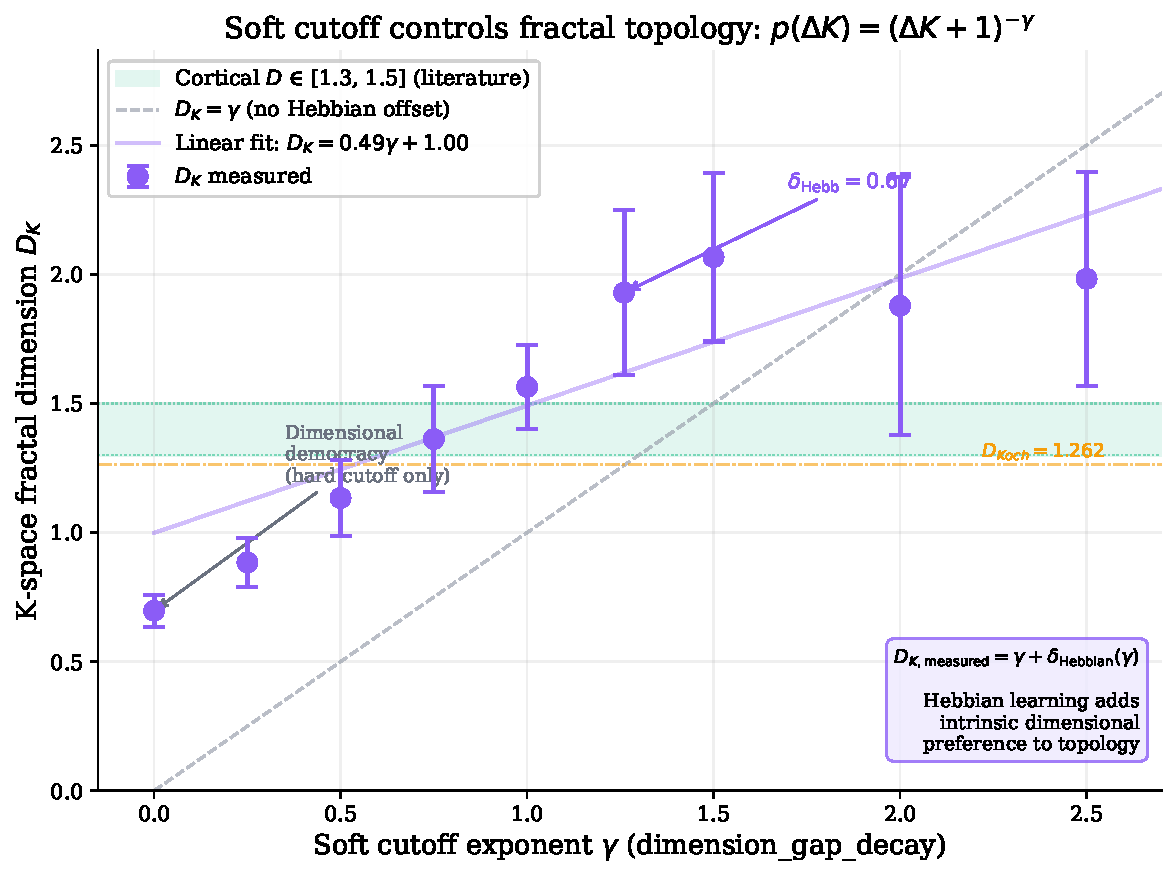
\includegraphics[width=\columnwidth]{../figures/fig3_dk_vs_gamma}
\caption{%
K-space fractal dimension $D_K$ vs.\ soft-cutoff exponent
$\gamma$.
Green band: cortical range $D \in [1.3, 1.5]$.
Purple line: fit $D_K = 0.76\gamma + 0.78$.
}
\label{fig:fractal}
\end{figure}


% ============================================================
%  PART B — FROM NETWORK TO BRAIN
% ============================================================

\part*{Part B: From Network to Brain}


% ============================================================
\section{Same-$K$ Clustering and Functional Regions}
\label{sec:clustering}
% ============================================================

Consider a network of neurons with heterogeneous $K$
values.
C2 gradient descent on the reflection action $A$
selectively strengthens same-$K$ edges
(more shared modes $\Rightarrow$ faster $\Gamma$ reduction
$\Rightarrow$ lower $A$) and weakens cross-$K$ edges
(excess modes totally reflected, no gradient available).
Under sustained activity plus edge pruning
(developmental apoptosis), the surviving connectivity
partitions the network into \emph{same-$K$ clusters}:
neurons sharing a common modal dimension self-segregate
into spatially contiguous aggregates.

The mechanism is thermodynamic phase separation:
MRP drives the system toward the lowest attainable $A$;
same-$K$ clustering minimises $\Acut$ at every internal
edge.

\begin{theorem}[Phase Separation Under MRP]
\label{thm:phase-sep}
Any impedance network under MRP with heterogeneous $K$
must phase-separate into same-$K$ domains to minimise
total reflected action.
\end{theorem}

\begin{proof}[Proof sketch]
For any edge connecting nodes with $K_i = K_j$,
$\Acut = 0$ on that edge.
For $K_i \neq K_j$, $\Acut = |K_i - K_j| > 0$.
Rewiring an edge from a cross-$K$ pair to a same-$K$
pair strictly reduces $\Acut$ (or leaves it unchanged if
no cross-$K$ edge exists).
C2 provides the dynamical mechanism: edges where all
modes converge ($\gamma_k \to 0$) are reinforced; edges
where excess modes are permanently reflected contribute
no gradient and are pruned under any activity-dependent
rule.
The fixed point of combined C2 + pruning is therefore a
graph where same-$K$ edges dominate.
\end{proof}

The mapping of specific $K$ ranges to specific
anatomical regions (sensory cortices, motor cortex,
prefrontal cortex, subcortical nuclei) is a
\emph{prediction} of this theorem, not an input;
its verification requires independent measurement of
neuronal modal complexity, which remains an open
experimental problem.


% ============================================================
\section{The Relay Hierarchy}
\label{sec:relay}
% ============================================================

Corollary~\ref{cor:relay} states that relay nodes are a
thermodynamic necessity.
In the nervous system, this produces a natural
$K$-level cascade:

\begin{center}
\begin{tabular}{lc}
\hline
\textbf{Level} & $K$ \\
\hline
Cortex (motor, sensory), thalamus & 5 \\
Spinal cord, motor/sensory neuron & 3 \\
Nociceptor A$\delta$ & 2 \\
Nociceptor C fibre & 1 \\
\hline
\end{tabular}
\end{center}

\noindent
The $K$ values are structural observations: a cortical
pyramidal cell has 5~physically distinct propagation
domains; a C-fibre has~1.
The theorem predicts that signals ascending from
$K = 1$ periphery to $K = 5$ cortex are stepped through
intermediate relays, recovering modes at each step.
Descending motor signals follow the same cascade in
reverse.

\subsection{Neural topology verification}
\label{sec:neural-topo}

A neural blueprint with 9~nodes spanning
$K \in \{5, 3, 2, 1\}$ and 12~directed edges
(descending motor, ascending sensory, and pain pathways)
was evolved for 300~ticks ($\eta = 0.02$, seed~$= 42$):
\begin{itemize}
  \item $\Aimp$ decays from $\sim\!1.79$ to zero.
  \item $\Acut$ rises from 9 (11~initial edges) to 37
    (60~edges), then saturates.
  \item The neural $\Acut$ at tick~1 ($= 9$) exceeds the
    cardiovascular $\Acut$ ($= 5$) because the neural
    topology has four $K$-levels vs.\ three,
    as predicted by Eq.~\eqref{eq:decomposition}.
\end{itemize}

\noindent
Full test suite: \texttt{tests/test\_e0\_neural.py}
(17~tests, 100\% pass).


% ============================================================
\section{The Brain as Convergence Region}
\label{sec:brain}
% ============================================================

An organism with multiple sensory modalities
(photoreceptors, mechanoreceptors, chemoreceptors,
thermoreceptors) has multiple ascending
pathways, each entering the network through a distinct
low-$K$ transducer.
For the organism to integrate information and produce
coordinated responses, these pathways must converge at
a common region.

By the irreducibility theorem, the convergence region
must satisfy
\begin{equation}
  K_{\text{conv}} \ge \max_j K_j
  \label{eq:K-convergence}
\end{equation}
for all input pathways~$j$; otherwise, modes from
higher-$K$ inputs are totally reflected and the
convergence region cannot process them.
The convergence region is therefore forced to be the
highest-$K$ cluster in the network.

This is the \emph{brain}: a topological necessity, not a
design choice.
Its properties follow from $K_{\text{conv}}$ being maximal:
\begin{itemize}
  \item \textbf{High metabolic cost.}
    Volumetric heat density scales as
    $q \propto K \cdot \avg{\Gamma^2} \cdot P_{\text{in}}$
    (Paper~0, Corollary~1~\cite{Paper0}).
    The brain's extreme $K$ concentrates a disproportionate
    share of metabolic heat in a small volume.
  \item \textbf{Temperature sensitivity.}
    Higher $K$ means more modes dissipating simultaneously;
    the Arrhenius thermal chain (Sec.~\ref{sec:thermo})
    makes the convergence region the most temperature-vulnerable
    tissue.
  \item \textbf{Matrix computation.}
    C2 gradient descent across all $K_{\text{conv}}$ modes
    simultaneously is the physical operation that
    neuroscience calls ``executive function''
    (Paper~4~\cite{Paper4}).
\end{itemize}

\noindent
The brain also serves as a ``hub'' connecting two
inter-organ buses: a vascular bus (delivering substrate
$\rho$) and a neural bus (distributing control signals).
The whole-body topology is detailed in Sec.~\ref{sec:whole-body}.


% ============================================================
\section{Signal Routing: Internal and External}
\label{sec:signals}
% ============================================================

C3 requires every signal to carry its source impedance
$Z_{\text{source}}$ as metadata.
In the nervous system, $Z_{\text{source}}$ is the
impedance of the transmitting neuron.
Different neuron types---photoreceptors,
mechanoreceptors, nociceptors, interoceptors---have
different physical structures and therefore different
impedance vectors.

At the convergence region, two routing cues are available
without any additional mechanism:
\begin{enumerate}
  \item \textbf{Relay-chain topology.}
    External signals enter through body-surface relay
    chains (skin $\to$ spinal dorsal horn $\to$ thalamus
    $\to$ cortex).
    Internal signals enter through visceral relay chains
    (organ $\to$ autonomic ganglion $\to$ brainstem
    $\to$ cortex).
    The two chains occupy distinct edges in the
    $\Gamma$-network; traversing different relay nodes
    means arriving at different input ports of the
    convergence region.

  \item \textbf{$Z_{\text{source}}$ metadata (C3).}
    Sensory neurons of different types carry
    distinguishable $Z$ signatures because their
    physical geometries differ.
    These signatures propagate through the relay chain;
    the convergence region receives them as C3 metadata
    and can route processing to the appropriate same-$K$
    cluster (Sec.~\ref{sec:clustering}).
\end{enumerate}

\noindent
The brain does not need a separate ``internal'' or
``external'' label; the impedance metadata and
relay-chain topology together provide full routing
information.
``Internal perception'' and ``external perception'' are
emergent properties of network topology and C3 transport,
not separate systems.

Descending signals follow the reverse path:
the convergence region generates motor or autonomic
commands that propagate through relay chains to
effectors.
The irreducibility theorem applies in both directions:
descending signals also lose modes at each $K$-step,
and relay nodes are equally necessary on the
efferent side.


% ============================================================
\section{Neural Pathology from Topology}
\label{sec:pathology}
% ============================================================

The irreducibility theorem has a direct clinical
implication: because $\Acut$ is determined by topology
(mode counts and edge structure) and has zero gradient
with respect to impedance, C2 cannot compensate for
topological damage.

This establishes a fundamental asymmetry:
\begin{itemize}
  \item \textbf{Impedance perturbation}
    (soft tissue injury, inflammation, transient chemical
    imbalance): C2 can repair, because $\Aimp$ is
    learnable.
    Given time, $\gamma_k \to 0$ on the perturbed edges.
  \item \textbf{Topological perturbation}
    (neuron death, axon severance, dendrite retraction):
    C2 cannot repair, because the change affects $\Acut$,
    which is invisible to the gradient.
\end{itemize}

\noindent
This is why brain damage is often permanent while soft
tissue heals.

\subsection{Edge severance (stroke)}

Removing an edge $i \to j$ eliminates a pathway.
Signals that traversed this edge are interrupted.
C2 can strengthen alternative pathways if they exist
(redundancy allows partial recovery), but the lost
edge's contribution to the network is permanently gone.
The deficit pattern is determined by \emph{which edge} is
lost: topology dictates which functions are impaired.

\subsection{Impedance escalation (ALS, demyelination)}

A diseased neuron's impedance $Z$ increases progressively.
At each of its edges, $\Gamma$ increases and $T$ decreases.
C2 attempts to compensate on neighbouring edges, but if
the disease is progressive ($Z$ continues to rise),
compensation cannot keep pace: the damaged node acts as
a growing impedance barrier that eventually isolates
itself from the network.

The neural topology test confirms this: ALS
(motor neuron $Z \times 3$) produces cumulative $\Aimp$
over 30~ticks that is $2.9\times$ the healthy baseline,
with descending motor signals progressively degraded
while sensory pathways remain intact---matching the
clinical pattern.

\subsection{Mode loss (neurodegeneration)}

A neuron that loses physical structure (spine retraction,
dendrite pruning) loses modes: $K_i$ decreases.
Previously matched edges (where $K_i = K_j$) now have
$\Acut > 0$.
This new irreducible cost appears abruptly and cannot be
removed by C2.
Cognitive decline is the progressive accumulation of
irreducible cost as neurons lose modes throughout the
convergence region.

\subsection{Pain as $\Gamma$-signal on low-$K$ pathways}

Tissue damage produces an abrupt local impedance
change, generating a $\Gamma$ spike on nociceptor edges.
Nociceptors sit at the lowest $K$ levels in the
hierarchy (C-fibre $K = 1$, A$\delta$ $K = 2$).
The $\Gamma$ spike propagates through the relay chain to
the convergence region.
Pain is not a special signal type---it is a high-$\Gamma$
event on a low-$K$ pathway.
Full treatment: Paper~4~\cite{Paper4}.

\subsection{Stroke verification}

The neural topology test confirms that severing the
cortex$\to$thalamus edge interrupts descending motor
transmission while the ascending sensory pathway remains
intact---the topology determines the deficit pattern
without any disease-specific code.


% ============================================================
%  PART C — FRACTAL COST OF MULTI-SCALE LIFE
% ============================================================

\part*{Part C: Fractal Cost of Multi-Scale Life}


% ============================================================
\section{Irreducible Action of a Self-Similar Relay Hierarchy}
\label{sec:acut-fractal}
% ============================================================

Part~A proved $\Acut > 0$ but left its geometric
structure unspecified.
Part~C asks: \emph{how big} is $\Acut$?

\subsection{Mode-count profile}

Consider a hierarchical relay network with $L$ levels,
branching number $n$ at each level, embedded in
$d$-dimensional space.
Level~0 is the root (e.g., aorta, cortex);
level~$L$ is the terminal (capillary, sensory ending).
At level~$\ell$:
number of nodes $N_\ell = n^\ell$;
segment length $l_\ell = l_0\,n^{-\ell/d}$ (space-filling);
mode count $K_\ell$.
Self-similar modelling:
\begin{equation}
  K_\ell = K_0\,c^\ell, \quad 0 < c < 1,
  \label{eq:mode-profile}
\end{equation}
with $c = n^{-1/d}$ when the cutoff is set by branch
length.

\subsection{$\Acut$ at each level}

From Theorem~\ref{thm:irreducibility}, the irreducible
action across an edge from level~$\ell$ to
level~$(\ell+1)$ is $(K_\ell - K_{\ell+1})^+$.
At level~$\ell$ there are $N_\ell = n^\ell$ such edges:
\begin{equation}
  \Acut = K_0(1 - c) \sum_{\ell=0}^{L-1} (nc)^\ell.
  \label{eq:acut-sum}
\end{equation}

\subsection{Scaling law}

With $c = n^{-1/d}$, the base of the geometric sum is
$nc = n^{(d-1)/d} > 1$ for $d \ge 2$, so the sum is
dominated by the last term:
\begin{equation}
  \boxed{\Acut \propto M^{(d-1)/d}.}
  \label{eq:acut-mass}
\end{equation}
\textbf{For $d = 3$:} $\Acut \propto M^{2/3}$.
The irreducible cost per cell is
$a_{\text{cut}} = \Acut / M \propto M^{-1/3}$,
which \emph{decreases} with organism size---economies of
scale from the relay hierarchy.

The K-space fractal dimension is
$D_K = \log n / \log(1/c) = d$.
The cortical $D_K \in [1.3, 1.5]$ measured in
Sec.~\ref{sec:fractal} reflects the cortex being a
folded sheet ($d_{\text{eff}} \approx 1.5$--$2$).


% ============================================================
\section{Murray's Ratio and Metabolic Scaling}
\label{sec:murray-kleiber}
% ============================================================

\subsection{The Murray bifurcation ratio}

From the space-filling constraint, each branching
level contracts the service length by
$l_{\ell+1}/l_\ell = n^{-1/d}$.
The bifurcation ratio:
\begin{equation}
  \boxed{\beta \equiv n^{1/d}.}
  \label{eq:beta-def}
\end{equation}
For binary bifurcation ($n = 2$) in $d = 3$:
\begin{equation}
  \beta = 2^{1/3} = 1.2599\ldots
  \label{eq:beta-value}
\end{equation}
From Murray's Law (Paper~2, Eq.~14~\cite{Paper2}):
$r_{\ell+1} = r_\ell / n^{1/3}$; for $d = 3$,
$r_{\ell+1} = r_\ell / \beta$.
Length and radius contract by the same ratio,
preserving the aspect ratio across the tree.

\subsection{Network maintenance cost}

The power dissipated by relay reflections is
$P_{\text{reflect}} = \Acut \cdot P_0 / N_T
\propto M^{(d-1)/d} \cdot M^{-1} = M^{-1/d}$.
Total network dissipation:
\begin{equation}
  B_{\text{network}} \propto M \cdot M^{-1/d}
  = M^{(d-1)/d}.
  \label{eq:B-network}
\end{equation}
For $d = 3$: $B_{\text{network}} \propto M^{2/3}$.

\subsection{Kleiber's Law}

Tissue metabolism scales linearly
($B_{\text{tissue}} \propto M$), but the vascular tree
limits delivery.
From the MRP perspective:
(1)~Murray's Law determines the radius ratio
$r_{\ell+1}/r_\ell = n^{-1/3}$;
(2)~space-filling determines the length ratio;
(3)~capillary invariance fixes the terminal scale;
(4)~blood volume $\propto M$.
Together: $N_T \propto M^{d/(d+1)}$ and therefore
\begin{equation}
  \boxed{B \propto M^{d/(d+1)}.}
  \label{eq:kleiber}
\end{equation}
For $d = 3$: $B \propto M^{3/4}$---Kleiber's
Law~\cite{Kleiber1932}, now a consequence of MRP.
The exponent decomposes as
$d/(d+1) = (d-1)/d + 1/[d(d+1)]$;
the extra $1/12$ arises from capillary invariance.

\subsection{Volumetric heat density and the $K$-bottleneck}

By Paper~0, Corollary~1~\cite{Paper0}, every active
interface dissipates $\Gamma_i^2 P_{\text{in},i}$ as heat.
A tissue with $K$ modes packs $K$ such interfaces into
one cross-section:
\begin{equation}
  q \propto K \cdot \avg{\Gamma^2} \cdot P_{\text{in}}
  / V_{\text{node}}\,.
  \label{eq:vol-heat}
\end{equation}
The human brain ($K = 5$) comprises $\sim$2\% of body mass
but generates $\sim$25\% of basal metabolic heat---not
despite being small, but \emph{because} its per-node mode
count is largest.
Kleiber's $M^{3/4}$ sets the whole-body envelope;
Eq.~\eqref{eq:vol-heat} sets the intra-body distribution,
concentrating heat where $K$ is highest and creating a
physical necessity for dedicated cerebral vasculature
(Paper~2~\cite{Paper2}).


% ============================================================
\section{Dual-Network Packing}
\label{sec:dual}
% ============================================================

\subsection{Two trees in one volume}

A multicellular organism requires two space-filling
networks: the \textbf{vascular tree}
($Z_v = \Delta P / Q$, transport) and the
\textbf{neural tree}
($Z_n = R_m + 1/j\omega C_m$, control).
Both must reach every cell.

\subsection{The packing theorem}

\begin{theorem}[Dual-Network Overhead]
\label{thm:packing}
When two space-filling relay trees share a volume in
$d$~dimensions,
\begin{equation}
  \Acut^{\text{dual}} = \Acut^v + \Acut^n + \Acouple,
  \quad \Acouple > 0.
  \label{eq:acut-dual}
\end{equation}
\end{theorem}

\begin{proof}
At co-terminal points, the two networks negotiate
resource allocation.
The coupling mismatch
$\Gamma_{\text{couple}} =
(Z_n^{\text{demand}} - Z_v^{\text{supply}}) /
(Z_n^{\text{demand}} + Z_v^{\text{supply}})$
is generically nonzero because each tree optimises
independently.
Hence $\Acouple = N_T \avg{\Gamma_{\text{couple}}^2} > 0$.
\end{proof}

\subsection{The metabolic overhead factor}

\begin{equation}
  \Omega \equiv \frac{B_{\text{total}}}{B_{\text{tissue}}}
  = 1 + \frac{B_{\text{vasc}} + B_{\text{neural}}}
             {B_{\text{tissue}}}.
  \label{eq:omega-def}
\end{equation}
For humans:
$B_{\text{neural}}/B_{\text{total}} \approx 0.20$
(brain~$\approx 20\%$ of BMR~\cite{Raichle2002});
$B_{\text{vasc}}/B_{\text{total}} \approx 0.05$.
Therefore
\begin{equation}
  \Omega \approx 1/0.75 \approx 1.33.
  \label{eq:omega-human}
\end{equation}
The neural network alone gives
$\Omega_n = 1/(1-0.20) = 1.25 \approx \beta = 2^{1/3}$.

\subsection{Why blood before nerve}

C2 requires a carrier for $x_{\text{in}}$: neurotransmitter
synthesis needs glucose and oxygen delivered by blood.
Without the vascular network, $x_{\text{in}} = 0$
everywhere, $\Delta Z = 0$: the neural network cannot
remodel.
Embryology confirms: cardiac tube at day~21; neural tube
closure at day~25--28.
In the product $1_v \times 1_n$, the vascular ``1'' is
the left factor.


% ============================================================
\section{Multi-Scale Verification}
\label{sec:multi-scale}
% ============================================================

The irreducibility theorem is not restricted to neural
tissue.
Every tissue where $K$ varies across an interface
produces $\Acut > 0$.
This section verifies the theorem across scales.

\subsection{Cardiovascular topology}
\label{sec:cv-topo}

An 11-node blueprint with $K$-levels
Cardiac Purkinje ($K = 4$) $\to$
vascular smooth muscle ($K = 2$) $\to$
endothelial ($K = 1$).
Over 300~ticks: $\Aimp \to 0$, $\Acut$ rises to~34 then
saturates, C1 holds at every edge.
Test: \texttt{tests/test\_e0\_cardiovascular.py}
(13~tests, 100\% pass).

\subsection{Joints as impedance relays}
\label{sec:joint}

A direct bone--synovial interface gives
$\Gamma = (120 - 50)/(120 + 50) = 0.54$, i.e.,
$T = 0.71$---nearly 30\% loss.
Cartilage at
$Z_{\text{cart}} \approx 80 \approx
\sqrt{Z_{\text{bone}} \cdot Z_{\text{syn}}}$
acts as a quarter-wave relay~\cite{Pozar2011},
achieving $T > 0.80$ per interface.
This is Corollary~\ref{cor:relay} in musculoskeletal form.
When cartilage degrades (osteoarthritis, $\eta \to 0$),
the relay is physically removed and $\Acut$ is no longer
mitigated.

\subsection{Twenty-nine tissue atlas}
\label{sec:tissue-atlas}

A comprehensive atlas of 29~organ-system blueprints
(Paper~0, Table~4~\cite{Paper0}) contains
$\sim$217~nodes, $\sim$242~directed edges, $K \in [1,5]$.
All 29 were verified under identical conditions
($\eta = 0.01$, 100~ticks): C1 holds, $\Aimp$ is
non-increasing, $\Acut$ is topologically invariant.
245~parametrised tests pass at 100\% rate
(\texttt{tests/test\_tissue\_blueprints.py}).

\subsection{Whole-body inter-organ topology}
\label{sec:whole-body}

The 29~blueprints are intra-organ networks.
Connecting them requires:
\begin{enumerate}
  \item \textbf{Vascular bus.}
    Aortic trunk ($K = 4$) $\to$ 29~arteriolar feeds
    ($K = 2$), $\Acut = 2$ per edge.
  \item \textbf{Neural bus.}
    Autonomic trunk ($K = 3$) $\to$ 29~nerve feeds
    ($K = 2$), $\Acut = 1$ per edge.
  \item \textbf{Brain hub.}
    Hypothalamus ($K = 3$) drives the neural bus;
    the vascular bus feeds interoceptive signals back
    to thalamus ($K = 5$).
\end{enumerate}

\noindent
The unified whole-body topology: 278~nodes, 426~edges,
$\Acut = 222$ (the structural information cost of
multi-organ life).
The total action:
\begin{equation}
  A_{\text{life}} = \Aimp^{\text{total}}(t)
  + \Acut^{\text{total}},
  \label{eq:A-life}
\end{equation}
where
\begin{equation}
  \Acut^{\text{total}} = \Acut^v + \Acut^n
  + \sum_{t=1}^{17} \Acut^t + \Acouple.
  \label{eq:acut-total}
\end{equation}
145~tests verify structure, C1/C2, bus connectivity,
and cross-organ signal propagation.

\subsection{Thermoregulation}
\label{sec:thermo}

Blood viscosity follows the Arrhenius law
$\tilde\eta(T) = \exp[\alpha(T^{-1} - T_0^{-1})]$
with $\alpha \approx 1949\,$K.
C2 repair slows by
$\tilde\eta_{\text{learn}}(T) = \exp[\beta_T(T_0^{-1}
- T^{-1})]$ with $\beta_T \approx 6015\,$K (enzymatic
Arrhenius).
Combined:
$\tilde\tau(T) = \exp[(\alpha+\beta_T)(T^{-1} - T_0^{-1})]$.
Setting $\tilde\tau(T_c) = \tau_{\max}$:
\begin{equation}
  T_c = \frac{T_0}{1 + T_0 \ln\tau_{\max} /
  (\alpha + \beta_T)}\,.
  \label{eq:Tc}
\end{equation}
Higher $K$ increases $\dot{Q} \propto K\,\Gamma^2$,
raising $T_c$:
$T_c(K{=}1) = -10.3\,^\circ$C (ectotherm viable);
$T_c(K{=}5) = +4.5\,^\circ$C (endothermy required).
93~tests verify the full chain
$\eta(T) \to Z \to \Gamma \to A[\Gamma]$.

\paragraph{Thermal refugia.}
During sleep ($P_{\text{basal}}$), if
$T_{\text{env}} < T_c(K) - P_{\text{basal}}\,R_{\text{th}}$,
the organism must couple to a high-heat-capacity mass
(burrow, tree hollow, conspecific huddle).
Endothermy \emph{and} thermal refugia both follow from
the same Arrhenius chain.

\paragraph{Surface insulation.}
The thermal balance
$\dot{Q}(K) = (T_{\text{body}} - T_{\text{env}})
/ R_{\text{th}}$ gives
\begin{equation}
  R_{\text{th}} = \frac{T_{\text{body}} - T_{\text{env}}}
  {\dot{Q}(K)}\,.
  \label{eq:Rth-K}
\end{equation}
High-$K$ organisms need low $R_{\text{th}}$ to shed
excess $\dot{Q}$; fur raises $R_{\text{th}}$; hence
fur reduction is forced once $K > K^*$ where
$\dot{Q}(K^*) R_{\text{th,fur}} > T_{\text{body}} - T_c$:
\begin{equation}
  K\!\uparrow
  \;\Rightarrow\;\dot{Q}\!\uparrow
  \;\Rightarrow\;R_{\text{th}}\text{ must }\downarrow\,.
  \label{eq:fur-loss-chain}
\end{equation}

\subsection{Geometric universality}
\label{sec:universality}

The ratio $\beta = n^{1/d}$ is a geometric inevitability
for any space-filling hierarchy---independent of
molecular substrate.
Vascular plants lack a neural network but obey Murray's
Law with $\beta = 2^{1/3}$~\cite{McCulloh2003} and
$B \propto M^{3/4}$~\cite{Niklas1994}, confirming $\beta$
is a property of geometry, not biology.
Plants have $\Omega \approx 1$ (no neural network);
the prediction
$\Omega_{\text{plant}} < \Omega_{\text{animal}}$ by
a factor approaching $\beta$ is testable by
cross-kingdom metabolic comparisons.


% ============================================================
\section{Discussion}
\label{sec:discussion}
% ============================================================

\subsection{Methodological caveat}

All numerical experiments in Part~A use simulation
modules built from C1--C3.
When the simulator confirms a theorem derived from those
axioms, it demonstrates \emph{internal consistency}, not
\emph{empirical validity}.
Only external measurements on biological impedance
networks can promote these results to physical truth.
The Part~C scaling laws are mathematical consequences of
the irreducibility theorem plus geometric constraints;
no simulation is involved.

\subsection{The concentric-circle structure}

This paper follows a strictly outward derivation:
single neuron $\to$ connectivity must exist $\to$
heterogeneous $K$ produces $\Acut$ $\to$ same-$K$
clustering $\to$ relay hierarchy $\to$ convergence
region (brain) $\to$ signal routing $\to$ pathology
$\to$ fractal cost $\to$ Kleiber's law.
Each step is a logical consequence of the previous;
no step requires information from a later one.
Biological nomenclature (``cortex'', ``stroke'',
``osteoarthritis'') is used for identification only---the
physics does not depend on it.

\subsection{Brain-scale feasibility}

$\tau_{\text{conv}} \sim N^{-1.12}$ predicts brain-scale
networks ($N \sim 10^{10}$) converge in
$\sim 10^{-11}$ ticks---effectively instantaneous.
The mechanism is mean-field averaging: effective field
strength grows with system size.
This prediction is measured at four sizes
only ($N \le 128$); brain-scale extrapolation should
be treated as a conjecture.

\subsection{What ``$1 \times 1 = \Omega$'' means}

Each ``1'' is a topologically one-dimensional tree in 3D.
Embedding imposes fractal cost; packing two trees adds
$\Acouple > 0$.
The result $\Omega \approx 1.25$--$1.33$ and the match
$\Omega_n \approx \beta$ suggest:
\emph{the cost of adding a second hierarchical tree is of
order one branching level of the first.}
This is empirically suggestive but not rigorously derived.

\subsection{Limitations}

\begin{enumerate}
  \item The self-similar mode profile
    (Eq.~\ref{eq:mode-profile}) is an idealisation;
    real networks have heterogeneous branching.
  \item The $K$ values for individual neuron types (5, 3,
    2, 1) are structural observations from counting
    propagation domains---not derived from C2.
    Independent validation (e.g., electrophysiological
    mode counting) is needed.
  \item The capillary invariance constraint is an
    empirical input; whether MRP alone determines the
    terminal scale is open.
  \item The Phase Separation Theorem
    (Theorem~\ref{thm:phase-sep}) assumes
    activity-dependent pruning; the specific pruning rule
    is not derived from C2.
\end{enumerate}


% ============================================================
\section{Falsifiable Predictions}
\label{sec:predictions}
% ============================================================

\begin{enumerate}
  \item \textbf{Same-$K$ clustering.}
    DTI-based grouping of axons by estimated mode count
    $K$ should yield spatial clustering that matches
    known functional regions.

  \item \textbf{Cortical fractal dimension.}
    Connectivity decay
    $p(\Delta K) \propto (\Delta K + 1)^{-\gamma}$ with
    $\gamma \approx 0.7$--$0.9$, yielding
    $D_K \in [1.3, 1.5]$ via Eq.~\eqref{eq:dk_fit}.

  \item \textbf{Vascular fractal dimension.}
    3D micro-CT should yield $d_H \to 3$ below capillary
    spacing (space-filling) and lower $d_H$ above.

  \item \textbf{Murray ratio invariance.}
    $\beta = 2^{1/3} \approx 1.26$ across all
    binary-branching species.

  \item \textbf{$\Omega$ across vertebrates.}
    Brain metabolic fraction should correlate with
    neural complexity:
    $\Omega_{\text{fish}} < \Omega_{\text{mammal}} <
    \Omega_{\text{primate}}$.

  \item \textbf{$\Omega \approx 1$ for plants.}
    $\Omega_{\text{plant}} \approx 1.05$.

  \item \textbf{Cartilage as relay.}
    $Z_{\text{cart}} \approx
    \sqrt{Z_{\text{bone}} \cdot Z_{\text{syn}}}$;
    osteoarthritic cartilage should show increased
    $\Gamma^2$.

  \item \textbf{Pathology--topology correlation.}
    Deficit patterns in stroke, ALS, and
    neurodegeneration should correlate with topological
    damage location, not with biochemical markers.

  \item \textbf{Signal-origin distinguishability.}
    Source impedance $Z_{\text{source}}$ should be
    measurably different across sensory modalities at
    the thalamic relay.

  \item \textbf{Embryonic geometry.}
    Fetal vasculature should show Murray-optimal
    $r_p / r_d \approx \beta$ from the earliest
    vasculogenesis (day~17--18).
\end{enumerate}


% ============================================================
\section{Conclusion}
\label{sec:conclusion}
% ============================================================

This paper derives neural architecture from a single
variational principle through eight logical steps:
\begin{enumerate}
  \item A single neuron under C2 requires $x_{\text{in}}$;
    connectivity is necessary.
  \item Heterogeneous $K$ produces the irreducibility
    theorem: $A = \Aimp(t) + \Acut$, with
    $\nabla_{\mathbf{Z}} \Acut \equiv 0$.
  \item C2's dimensional preference forces same-$K$
    clustering---functional regions.
  \item The irreducibility corollary makes relay nodes a
    thermodynamic necessity---layered hierarchy.
  \item Multi-modal convergence forces
    $K_{\text{conv}} \ge \max K_j$---the brain.
  \item C3 metadata $+$ relay-chain topology provide
    signal routing---internal vs.\ external perception.
  \item Topological invariance of $\Acut$ makes
    structural damage irreversible---neural pathology.
  \item Fractal cost $\Acut \propto M^{2/3}$, Murray's
    $\beta = 2^{1/3}$, and $B \propto M^{3/4}$---metabolic
    scaling.
\end{enumerate}

\noindent
The title equation is now precise:
\begin{equation}
  1_v \times 1_n = \Omega \approx \beta
  = 2^{1/3} \approx 1.26.
\end{equation}
Life pays a fractal tax of $\beta - 1 \approx 26\%$---the
price of one extra branching level, expressed as the
brain's share of the metabolic budget---for the privilege
of being simultaneously fed and informed.


\begin{acknowledgments}
The author thanks the open-source scientific Python
community (NumPy, SciPy, Matplotlib).
Simulations were performed on a personal workstation.
\end{acknowledgments}


% ============================================================
%  BIBLIOGRAPHY
% ============================================================
\begin{thebibliography}{99}

\bibitem{Paper0}
H.-Y.~Huang,
``Paper~0: The $\Gamma$-Net Framework---Impedance Physics
for Electronic Lifeforms,''
preprint (2026).

\bibitem{Paper2}
H.-Y.~Huang,
``Paper~2: Dual Impedance Networks---Vascular and Neural
Organ Health from the Minimum Reflection Principle,''
preprint (2026).

\bibitem{Paper3}
H.-Y.~Huang,
``Paper~3: Temporal Dynamics---Impedance Debt, Sleep,
Lifecycle, and Aging,''
preprint (2026).

\bibitem{Paper4}
H.-Y.~Huang,
``Paper~4: Memory, Consciousness, and Nociception as
Impedance Physics on the $\Gamma$-Net,''
preprint (2026).

\bibitem{Paper5}
H.-Y.~Huang,
``Paper~5: The Grand Unification---$\Gamma$ as the
Universal Interface Law from Microtubules to Power Grids,
and C2 as Universal Remodeling in Twenty-Nine Tissues,''
preprint (2026).

\bibitem{HH1952}
A.~L.~Hodgkin and A.~F.~Huxley,
J.~Physiol.\ \textbf{117}, 500 (1952).

\bibitem{Breakspear2017}
M.~Breakspear,
Nat.\ Neurosci.\ \textbf{20}, 340 (2017).

\bibitem{cortex_fractal}
T.~G.~Smith \textit{et al.},
J.~Comp.\ Neurol.\ \textbf{323}, 48 (1992);
R.~D.~King \textit{et al.},
NeuroImage \textbf{56}, 1838 (2011).

\bibitem{Pozar2011}
D.~M.~Pozar, \emph{Microwave Engineering}, 4th~ed.\
(Wiley, 2011).

\bibitem{WBE1997}
G.~B.~West, J.~H.~Brown, and B.~J.~Enquist,
Science \textbf{276}, 122 (1997).

\bibitem{Kleiber1932}
M.~Kleiber,
Hilgardia \textbf{6}, 315 (1932).

\bibitem{McCulloh2003}
K.~A.~McCulloh, J.~S.~Sperry, and F.~R.~Adler,
Nature \textbf{421}, 939 (2003).

\bibitem{Niklas1994}
K.~J.~Niklas,
\emph{Plant Allometry} (Univ.\ Chicago Press, 1994).

\bibitem{Raichle2002}
M.~E.~Raichle and D.~A.~Gusnard,
Proc.\ Natl.\ Acad.\ Sci.\ USA \textbf{99}, 10237 (2002).

\bibitem{ALICE_code}
H.-Y.~Huang,
``Alice Smart System---Gamma-Net reference implementation,''
\url{https://github.com/cyhuang76/alice-gamma-net} (2026).

\end{thebibliography}

\end{document}
